\chapter{SYSTEM DESIGN }

 \section{Use case model}
\begin{figure}[H]
    \centering
    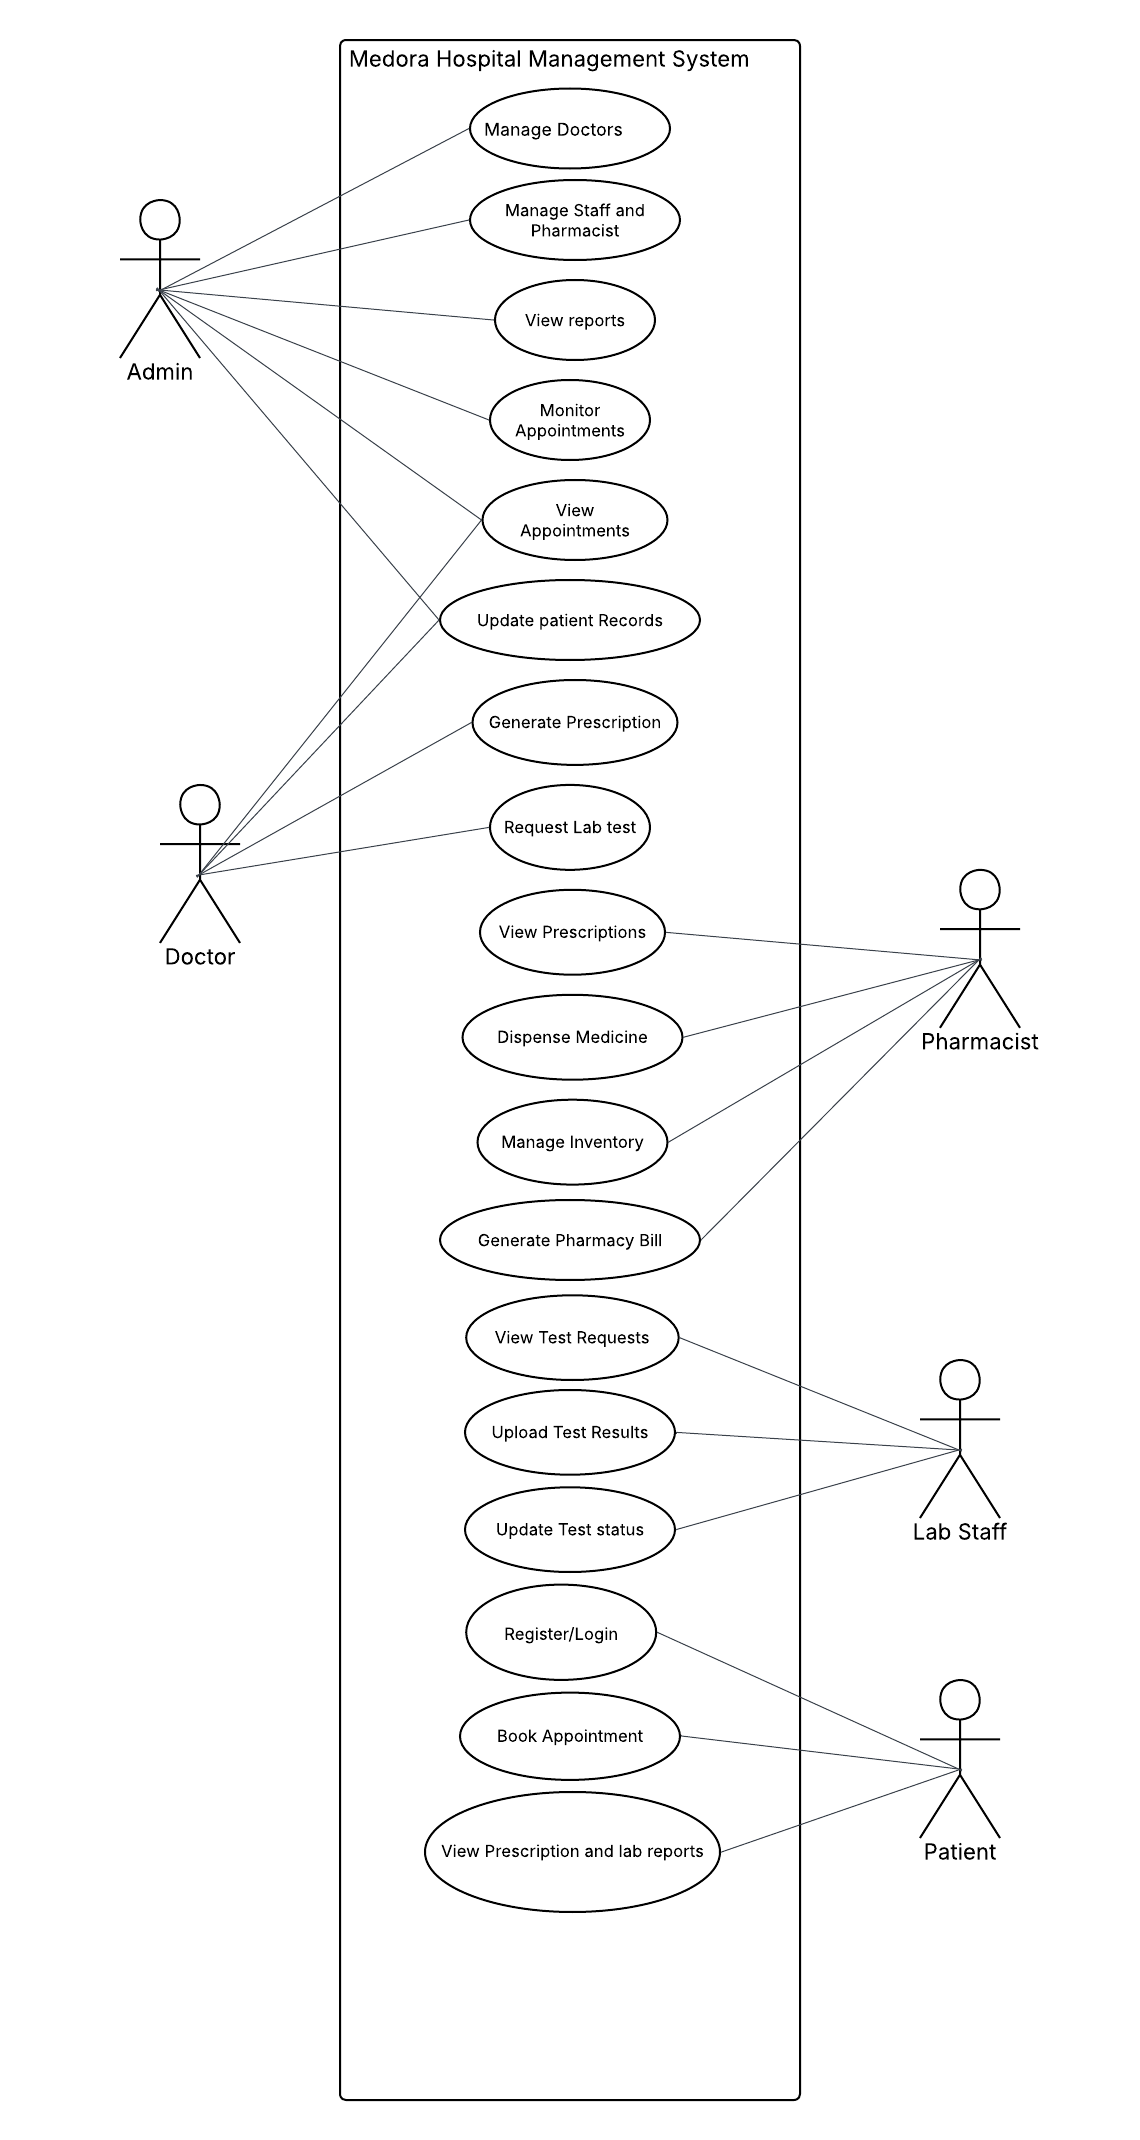
\includegraphics[width=1\textwidth,height=0.9\textwidth]{Blank diagram.png}
    \caption{Use case Diagram}
    \label{fig:Use_case}
\end{figure}
This Use Case Diagram illustrates the interactions between users and the Medora Hospital Management System. The Admin manages doctors, staff, appointments, patient records, and reports. The Doctor conducts consultations, generates prescriptions, and requests lab tests. The Pharmacist verifies prescriptions, dispenses medicines, manages inventory, and generates pharmacy bills. The Lab Staff handles test requests, uploads results, and updates test status. The Patient can register/login, book appointments, and view prescriptions and lab reports.
 \section{Activity Diagram}
 \subsection{Appointment Booking}
\begin{figure}[H]
    \centering
    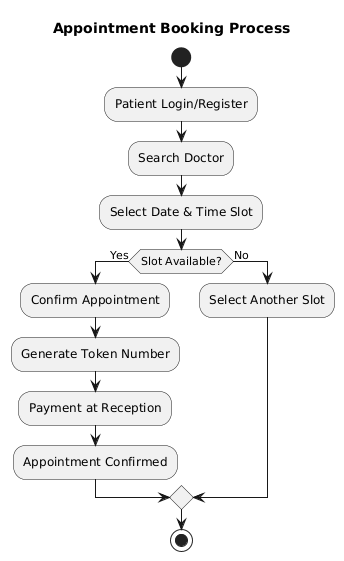
\includegraphics[width=1\textwidth,height=0.9\textwidth]{appoinmentBooking_activity.png}
    \caption{Appointment Booking Activity diagram}
    \label{fig:Use_case}
\end{figure}
This Activity Diagram represents the Appointment Booking Process in the Medora Hospital Management System. The process begins when the patient logs in or registers in the system. The patient then searches for a doctor and selects a preferred date and time slot.The system checks whether the selected slot is available. If the slot is available, the patient confirms the appointment, a token number is generated, and payment is made at the reception. Finally, the appointment is successfully confirmed.If the slot is not available, the patient is prompted to select another time slot before proceeding.\subsection{Consultation and Prescription}
\begin{figure}[H]
    \centering
    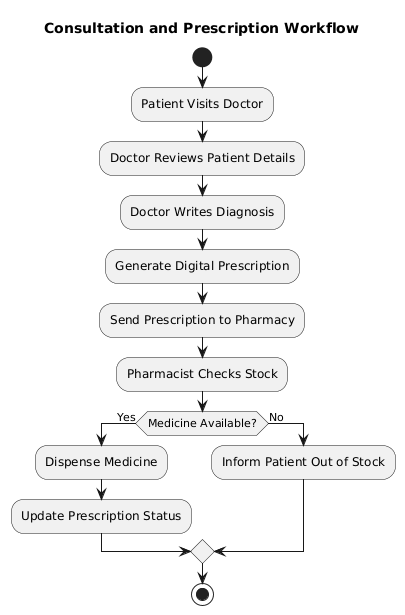
\includegraphics[width=0.5\textwidth]{Consultation_Prescription_activity.png}
    \caption{Consultation and Prescription Activity Diagram}
    \label{fig:Use_case}
\end{figure}
This Activity Diagram (Figure 3.3) represents the Consultation and Prescription workflow of the Medora Hospital Management System. The process begins when a patient visits the doctor or attends a scheduled appointment. The doctor reviews the patient’s details and medical history before conducting the consultation and recording the diagnosis.After evaluation, the doctor generates a digital prescription within the system. The prescription is then made available to the pharmacy module for processing. The pharmacist checks medicine availability in the inventory.If the prescribed medicines are available, the pharmacist dispenses the medicines to the patient and updates the prescription status in the system. If the medicines are not available, the pharmacist informs the patient about the out-of-stock items. Finally, the prescription status is updated accordingly, completing the workflow.
\subsection{Direct Pharmacy Purchase}

\begin{figure}[H]
    \centering
    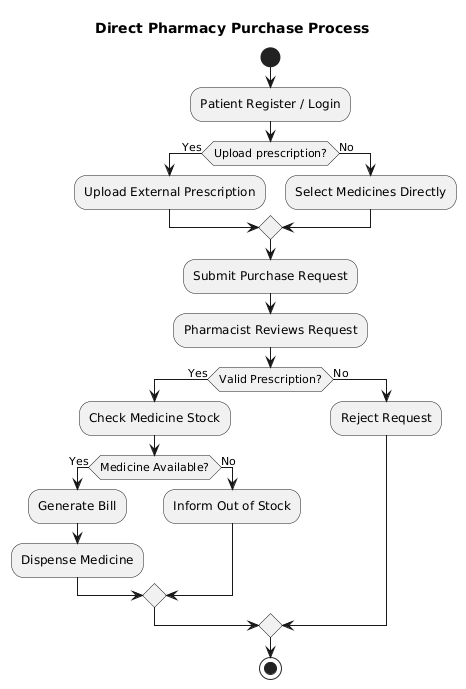
\includegraphics[width=0.7\textwidth]{Direct_Pharmacy_activity.png}
    \caption{Direct Pharmacy Purchase Activity Diagram}
    \label{fig:Use_case}
\end{figure}

This Activity Diagram represents the Direct Pharmacy Purchase workflow in the Medora Hospital Management System. The process begins when a patient logs into the system and chooses to purchase medicines from the pharmacy module without undergoing a doctor consultation.The patient can either upload an external prescription or directly select medicines from the available inventory. Once the purchase request is submitted, the pharmacist reviews the prescription or medicine request.If a prescription is uploaded, the pharmacist verifies its validity before proceeding. The pharmacist then checks the availability of the requested medicines in the inventory.If the medicines are available in stock, the system generates a bill and the pharmacist dispenses the medicines to the patient. The stock quantity is automatically updated in the database. If the prescription is invalid or the medicines are out of stock, the pharmacist rejects the request or informs the patient accordingly. This workflow ensures secure medicine dispensing, proper stock management, and accurate billing without mandatory doctor consultation.
\section{Sequence Diagram}

\subsection{Appointment Booking}

\begin{figure}[H]
    \centering
    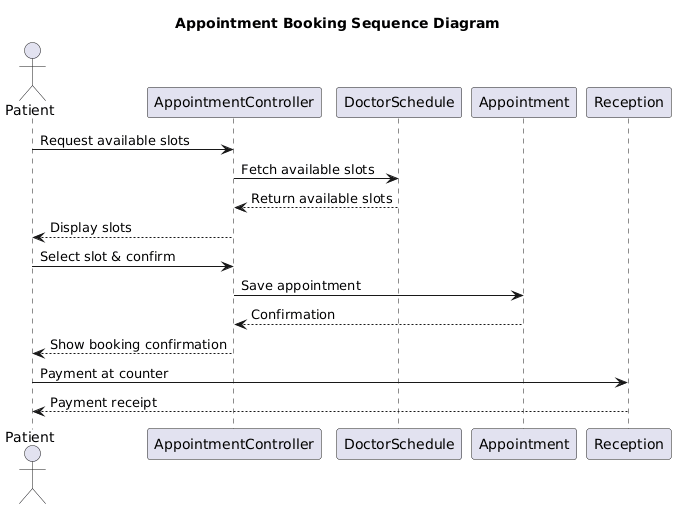
\includegraphics[width=0.9\textwidth]{AppointmentBookingSD.png}
    \caption{Appointment Booking Sequence Diagram}
    \label{fig:Use_case}
\end{figure}

This sequence diagram illustrates the interaction between Patient, Appointment Controller, Doctor Schedule, and Reception during the appointment booking process. The process begins when the patient logs in and searches for available doctors. The system checks doctor availability and returns available time slots. The patient selects a preferred slot and confirms the appointment. The appointment controller validates the slot and stores the booking details in the database. Finally, the reception processes the payment and confirms the appointment.

\subsection{Consultation and Prescription}

\begin{figure}[H]
    \centering
    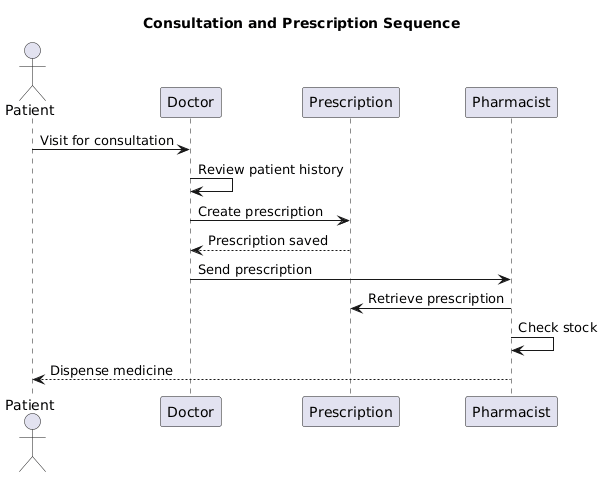
\includegraphics[width=0.9\textwidth]{Consulation_Prescription_SD.png}
    \caption{Consultation and Prescription Sequence Diagram}
    \label{fig:Use_case}
\end{figure}

This sequence diagram represents the interaction between Patient, Doctor, Prescription Module, and Pharmacist during a consultation. After the patient visits the doctor, the doctor reviews the medical details and enters the diagnosis into the system. The system generates a digital prescription and stores it in the database. The pharmacist retrieves the prescription, checks medicine availability, and dispenses the medicines. The prescription status is updated accordingly.

\subsection{Direct Pharmacy Purchase}

\begin{figure}[H]
    \centering
    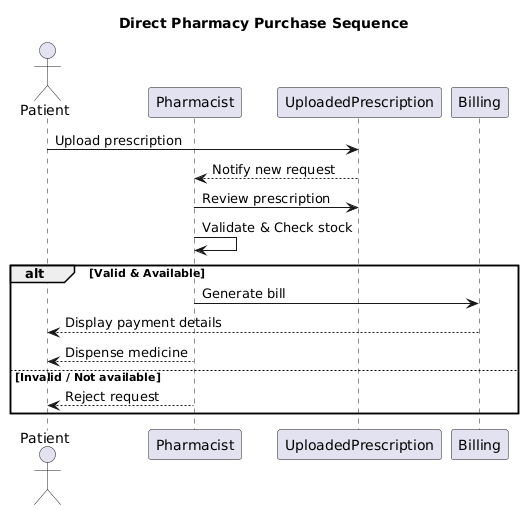
\includegraphics[width=0.9\textwidth]{DirectPharmacySD.png}
    \caption{Direct Pharmacy Purchase Sequence Diagram}
    \label{fig:Use_case}
\end{figure}

This sequence diagram explains the direct pharmacy purchase process without doctor consultation. The patient logs in and either uploads an external prescription or directly selects medicines. The request is sent to the pharmacist for verification. The pharmacist validates the prescription (if uploaded) and checks stock availability. If approved, the billing module generates an invoice and the medicines are dispensed. The stock quantity is updated in the database. If the prescription is invalid or medicines are unavailable, the request is rejected.

\section{Project Design}

System design is the process of defining the architecture, components, modules, interfaces, and data flow of a system to meet specified requirements. It ensures that the system is structured, scalable, secure, and user-friendly. Good system design focuses on usability, efficiency, performance, and data security while maintaining clear role-based responsibilities and workflow management. 

In Medora Hospital Management System, the system design focuses on integrating multiple hospital departments such as Administration, Reception, Doctors, Pharmacy, and Laboratory into a centralized digital platform. The design ensures smooth patient registration, appointment scheduling, prescription management, laboratory processing, and billing operations. The system balances operational efficiency and patient convenience by implementing role-based dashboards, secure data handling, and real-time updates.

\subsection{UI Design}

The User Interface (UI) design of Medora Hospital Management System is structured to be clean, intuitive, and role-specific. Each user type—Admin, Receptionist, Doctor, Pharmacist, Lab Staff, and Patient—has a dedicated dashboard displaying relevant features and information.

The UI includes:
\begin{itemize}
    \item Login and registration screens with secure authentication.
    \item Appointment booking forms with date and time slot selection.
    \item Doctor dashboard displaying scheduled appointments and patient details.
    \item Pharmacy interface for prescription verification and medicine dispensing.
    \item Laboratory interface for updating test results and status.
    \item Billing interface for invoice generation and payment tracking.
\end{itemize}

The interface ensures smooth navigation, clear layout, and easy access to system functionalities, improving overall hospital workflow efficiency.

\subsection{User Interaction Design}

The system is designed to provide responsive and user-friendly interaction across all modules. Each action such as booking appointments, generating prescriptions, uploading lab reports, or dispensing medicines triggers real-time validation and updates.

Role-based interaction ensures:
\begin{itemize}
    \item Patients can register, book appointments, view prescriptions, upload external prescriptions, and purchase medicines.
    \item Doctors can review patient records, enter diagnoses, and generate prescriptions.
    \item Receptionists can manage bookings and billing.
    \item Pharmacists can verify prescriptions and manage inventory.
    \item Lab staff can update test reports securely.
\end{itemize}

The system prevents unauthorized access and ensures smooth transitions between processes such as appointment confirmation, prescription validation, and billing completion.

\subsection{Billing and Transaction Design}

The billing system is structured to automatically generate invoices for:
\begin{itemize}
    \item Doctor consultations
    \item Laboratory tests
    \item Medicine purchases
\end{itemize}

The total amount is calculated dynamically based on services provided. Payment status is recorded and updated within the system. This ensures financial transparency and accurate transaction tracking.

\subsection{Database Design}

The database design follows a relational structure using MySQL. Key entities include:

\begin{itemize}
    \item User
    \item Doctor
    \item Patient
    \item Appointment
    \item Prescription
    \item Medicine
    \item LabTest
    \item Billing
\end{itemize}

Each entity is linked using foreign key relationships to maintain data consistency and avoid duplication. The structured database ensures secure storage and efficient retrieval of hospital records.

\subsection{Workflow Design}

The system workflow ensures smooth hospital operations:

\begin{itemize}
    \item Patient registers in the system.
    \item Appointment is booked via Reception or Patient dashboard.
    \item Doctor conducts consultation and generates prescription.
    \item Lab tests are requested if required.
    \item Pharmacist dispenses medicines based on prescription.
    \item Billing is generated and payment status is updated.
    \item Alternatively, patient can upload an external prescription and directly purchase medicines from pharmacy.
\end{itemize}

\subsection{System Screenshots}

\begin{figure}[H]
    \centering
    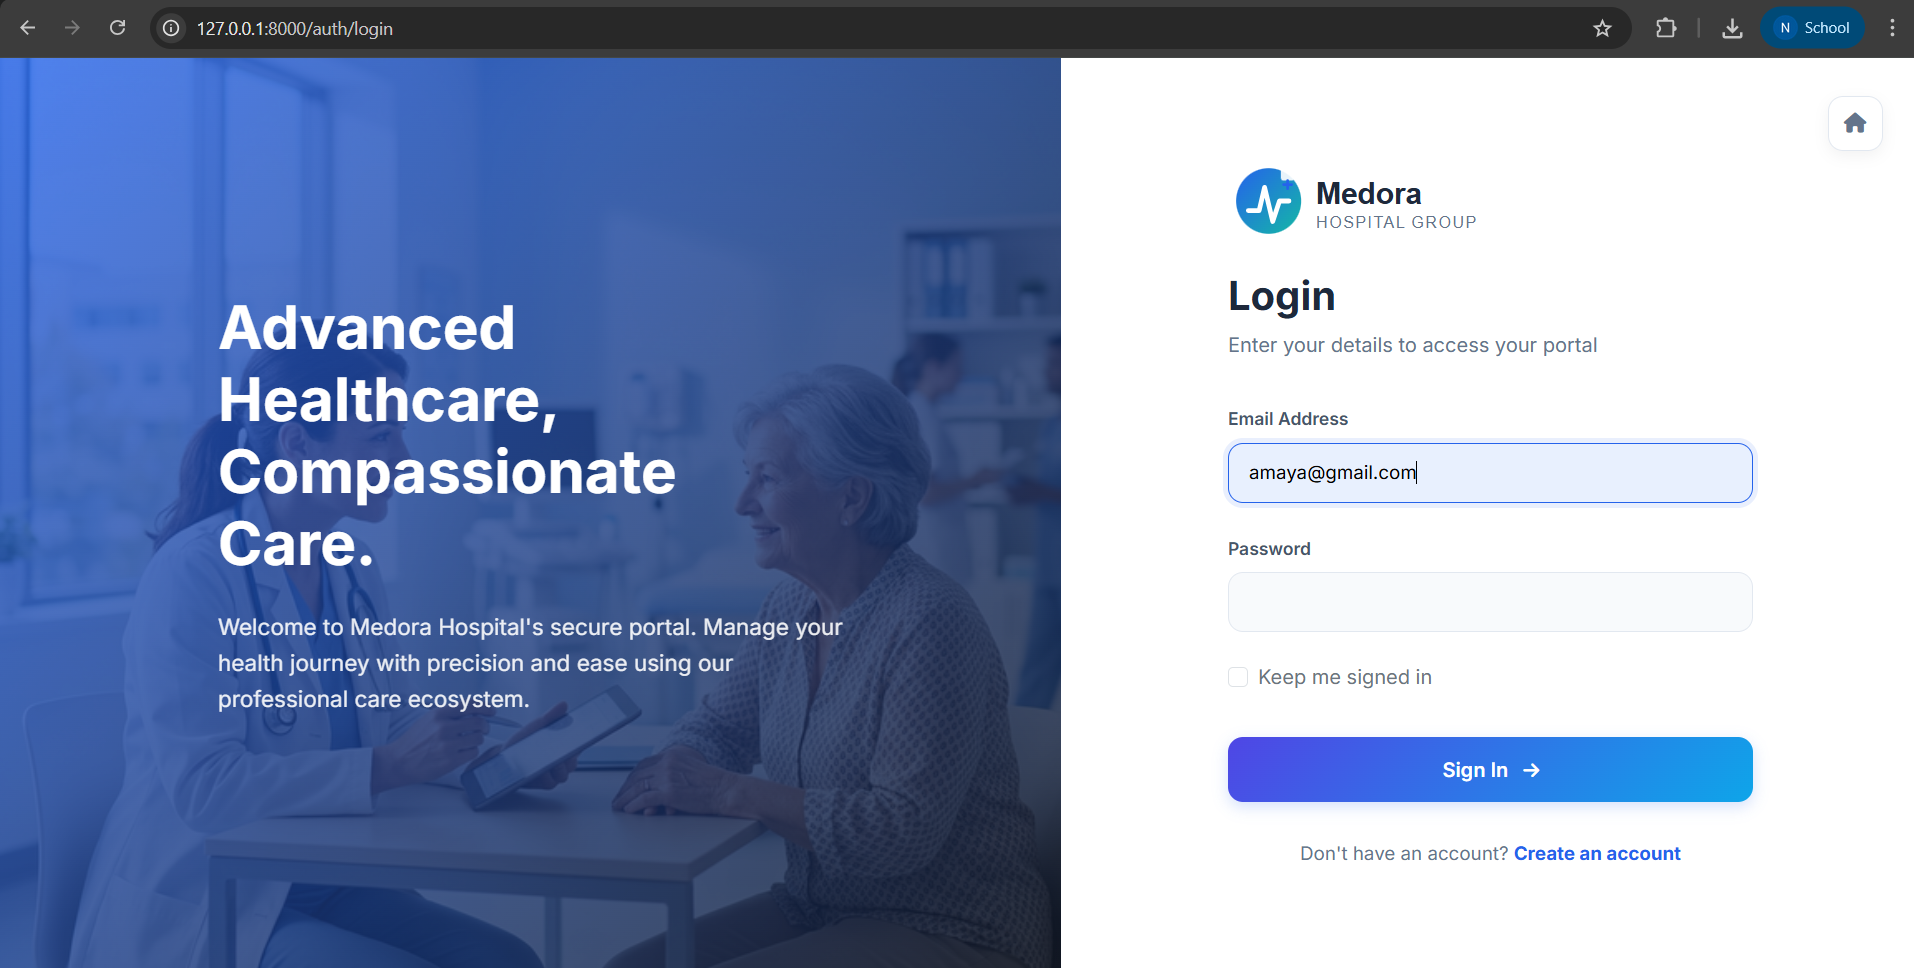
\includegraphics[width=0.9\textwidth]{login.png}
    \caption{Login Interface}
    \label{fig:Use_case}
\end{figure}

\begin{figure}[H]
    \centering
    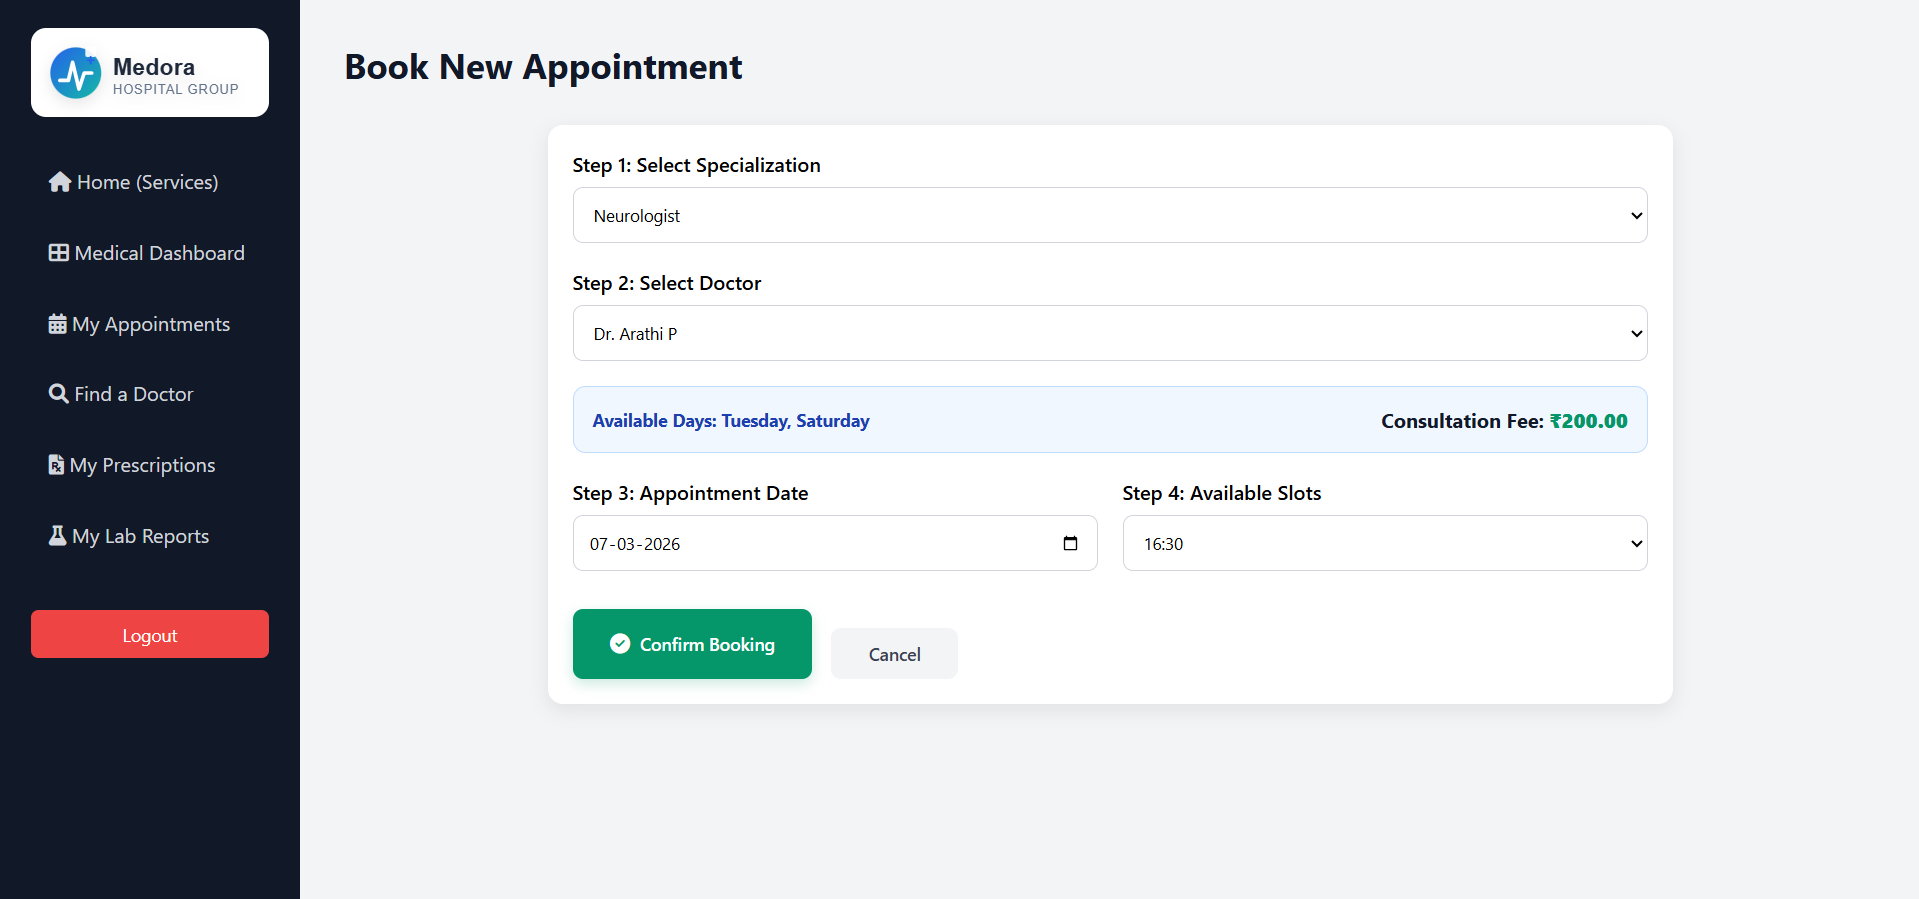
\includegraphics[width=0.9\textwidth]{Screenshot 2026-03-02 012323.png}
    \caption{Appointment Dashboard}
    \label{fig:Use_case}
\end{figure}

\begin{figure}[H]
    \centering
    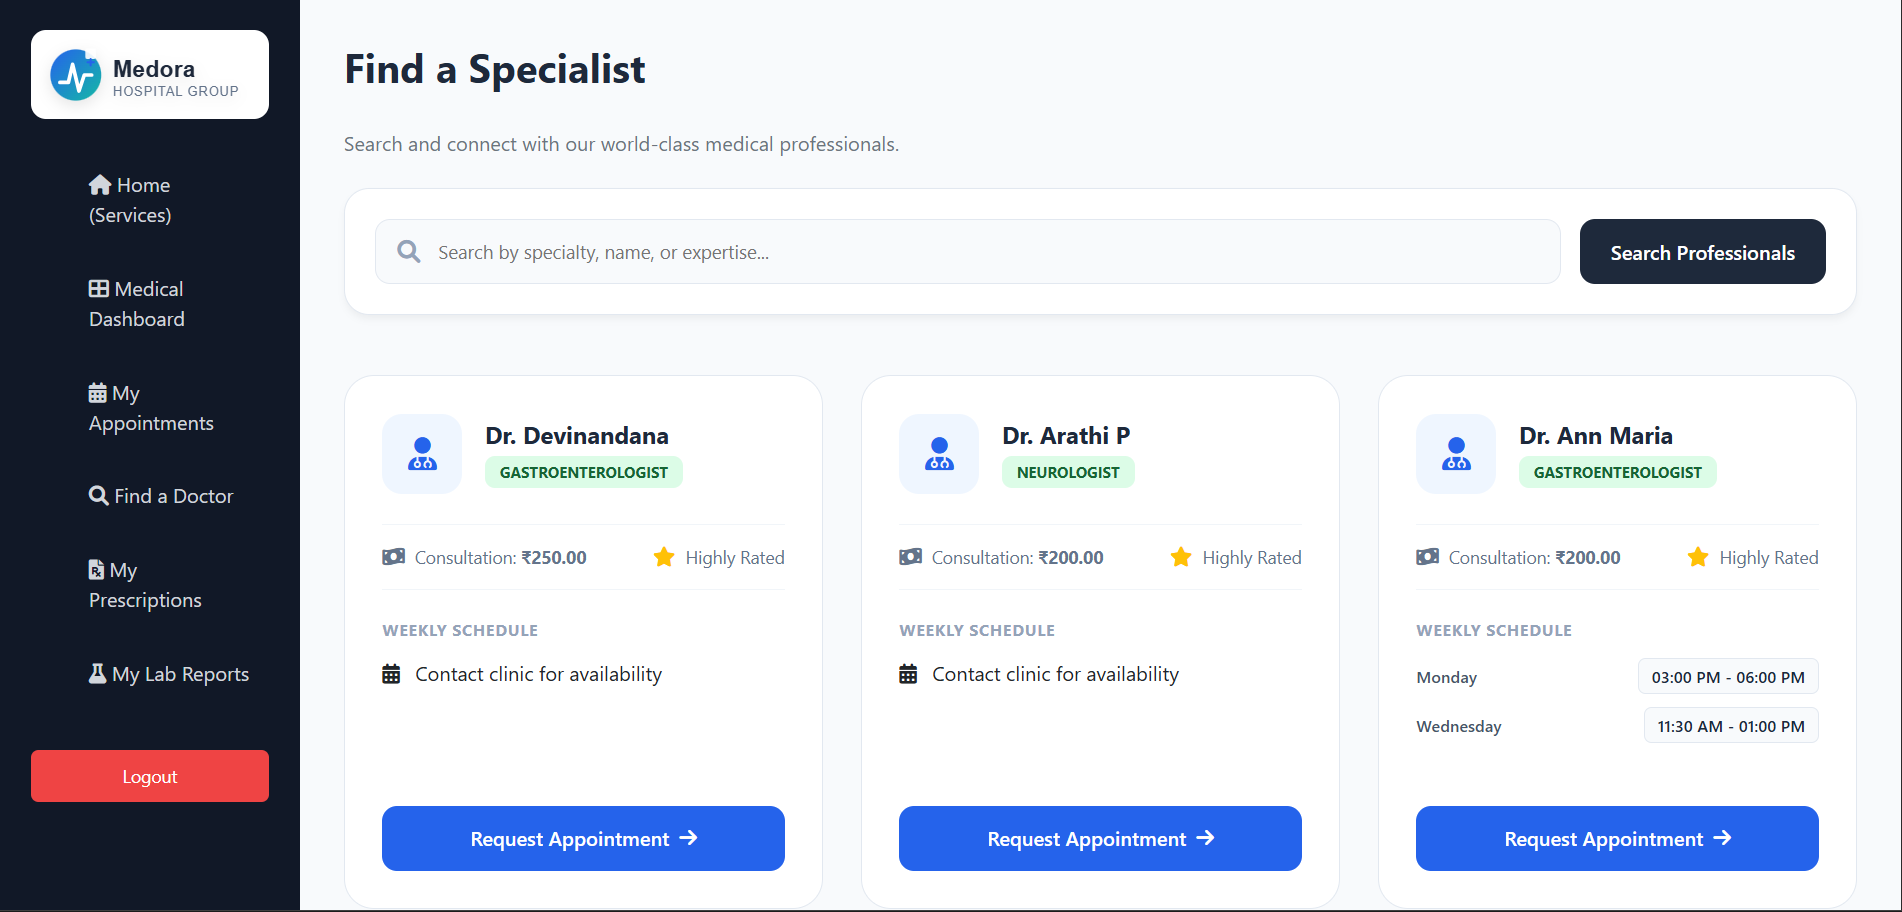
\includegraphics[width=0.9\textwidth]{finddoctor.png}
    \caption{Doctor Search}
    \label{fig:Use_case}
\end{figure}

\subsection{Data Structure Design}

Hospital data is stored in structured database tables rather than JSON format. Each record includes key attributes such as:

\begin{itemize}
    \item Patient personal details
    \item Doctor specialization and availability
    \item Appointment date and token number
    \item Prescription details and status
    \item Lab test results and remarks
    \item Billing amount and payment status
\end{itemize}

The structured design ensures scalability, maintainability, and data integrity throughout the system.